% =====================================================================
% Reporte técnico de experimentos — anexo técnico de la ENTREGA FINAL
% Proyecto Aplicado en Analítica de Datos (MIAD)
%
% Evoluciona a partir de reporte_tecnico_experimentos.tex (Módulo 2, 97/100),
% que queda congelado como registro de lo calificado. Incorpora la
% retroalimentación de esa entrega y de la anterior: explicación de los
% umbrales por cuantiles (§5.1), Apéndice A (colinealidad) y Apéndice B
% (configuración de parámetros, leída de los modelos y del código).
% Las tablas de los apéndices las genera reports/apendices/generar_apendices.py.
%
% Las figuras se leen de ./figures/ (rutas relativas a este archivo).
% Compilar: tectonic reporte_tecnico_final.tex  (o subir a Overleaf).
% =====================================================================
\documentclass[11pt,a4paper]{article}

\usepackage[utf8]{inputenc}
\usepackage[T1]{fontenc}
\usepackage{lmodern}
% NOTA: los signos de apertura se escriben como \textquestiondown{} y
% \textexclamdown{}; el carácter literal no se compone bien con esta
% combinación de codificación y fuentes.
\usepackage[spanish,es-nodecimaldot,es-noshorthands]{babel}
\usepackage[margin=2.5cm]{geometry}
\usepackage{float}
\usepackage{booktabs}
\usepackage{graphicx}
\usepackage{longtable}
\usepackage{array}
\usepackage{xcolor}
\usepackage{caption}
\usepackage{enumitem}
\usepackage{tikz}
\usetikzlibrary{arrows.meta, positioning, shapes.geometric}
\usepackage[hidelinks]{hyperref}

\captionsetup{font=small, labelfont=bf}
\setlist{itemsep=2pt, topsep=3pt}
\renewcommand{\arraystretch}{1.15}
\emergencystretch=1.5em
\hyphenation{His-t-Gra-dient-Boos-ting In-ter-pre-ta-bi-li-dad re-que-ri-mien-to}

% Columnas de ancho fijo con alineación superior
\newcolumntype{L}[1]{>{\raggedright\arraybackslash}p{#1}}
\newcolumntype{C}[1]{>{\centering\arraybackslash}p{#1}}

\title{\vspace{-1.2cm}\textbf{Reporte técnico de experimentos}\\[0.25cm]
\large Detección de tráfico de red malicioso mediante clasificación\\
\large con desbalance extremo de clases e interpretabilidad\\
\large \vspace{0.3cm} Proyecto Aplicado en Analítica de Datos --- Entrega final\\
\normalsize Anexo técnico (ii): implementación y experimentos del prototipo}
\author{Mariana Pérez\\Bryan Rodriguez\\Daniela Zúñiga}


\begin{document}
\maketitle
\thispagestyle{empty}

\begin{abstract}
\noindent
Este reporte documenta la implementación y los experimentos del prototipo de
detección de tráfico de red malicioso sobre el conjunto de datos CIC-IDS2017.
Se describen: (i) los modelos seleccionados y su correspondencia con los
requerimientos aprobados; (ii) las alternativas evaluadas con sus ventajas y
desventajas; (iii) la verificación de los supuestos de cada familia de
modelos y el tratamiento previo de los datos que cada una exige; (iv) el
protocolo de entrenamiento, validación y parametrización, con la
justificación de las métricas empleadas; (v) el análisis de resultados y los
ajustes implementados a partir de él; y (vi) el estado de implementación del
prototipo y el plan para completarlo. El modelo seleccionado alcanza un
macro-F1 de 0,975 sobre el conjunto de prueba, manteniendo las falsas alarmas
en 0,12\% del tráfico benigno; la estimación conservadora, que no depende del
puerto de destino, es de 0,942.
\end{abstract}

\vspace{0.3cm}

% =====================================================================
\section{Contexto y alcance}
% =====================================================================

\textbf{Problema:} Un centro de operaciones de seguridad (SOC) recibe cientos
de miles de \emph{flujos de red} por día. Un flujo es una conversación entre
dos computadores resumida en medidas numéricas (cuántos paquetes, de qué
tamaño, con qué ritmo, cuánto duró), sin acceso al contenido de la
comunicación. Revisarlos manualmente es inviable y las reglas por firma no
reconocen ataques nuevos.

\textbf{Usuario objetivo:} Analista de seguridad de un SOC. Conoce redes y
tipos de ataque, pero no es científico de datos ni programador, y sobre todo
se enfrenta a un volumen de tráfico que ninguna persona puede revisar
manualmente. Necesita \emph{priorizar} qué flujos investigar y disponer de una
razón que pueda justificar ante terceros.

\textbf{Datos:} CIC-IDS2017 (Canadian Institute for Cybersecurity;
Sharafaldin et al., 2018): una semana
simulada de tráfico corporativo, con 2.830.743 flujos etiquetados como
benignos (80,3\%) o como uno de 14 tipos de ataque (19,7\%). El desbalance es
extremo: la clase más frecuente supera a la más rara en una razón de
206.645 a 1.

\textbf{Encuadre analítico:} El problema se aborda como uno de
\textbf{clasificación con desbalance de clases e interpretabilidad}, no como
un problema de seguridad ofensiva.

% =====================================================================
\section{Modelos propuestos y su correspondencia con los requerimientos}
% =====================================================================

\subsection{Requerimiento al modelo}

Los requerimientos aprobados se agrupan en tres preguntas analíticas, y cada
una determina una familia de modelos distinta, donde el
Cuadro~\ref{tab:req-modelo} hace esa correspondencia explícita.

\begin{table}[H]
\centering
\caption{Correspondencia entre requerimientos, pregunta analítica y modelo.}
\label{tab:req-modelo}
\footnotesize\setlength{\tabcolsep}{4pt}
\begin{tabular}{L{1.5cm} L{4.3cm} L{3.6cm} L{4.6cm}}
\toprule
\textbf{Req.} & \textbf{Requerimiento} & \textbf{Pregunta analítica} & \textbf{Modelo que responde} \\
\midrule
R1, R6, R14 & Clasificar el tipo de ataque pese al desbalance, con desempeño accionable &
\textquestiondown{}De qué tipo es este ataque? & Clasificador multiclase supervisado (11 clases) \\
R2 & Reducir falsas alarmas para disminuir la fatiga de alertas &
\textquestiondown{}Cuántas alarmas falsas genera? & El mismo multiclase, evaluado por precisión y recall por clase \\
R3 & Explicar en qué se basa el modelo &
\textquestiondown{}Por qué se marcó esta alerta? & Técnicas de interpretabilidad aplicadas al clasificador: lectura global e individual \\
R4 & Detectar comportamientos anómalos no etiquetados &
\textquestiondown{}Esto es raro, aunque no sepa qué es? & Detector de anomalías no supervisado \\
R5 & Demostrar valor frente al escenario sin herramienta &
\textquestiondown{}Cuánto trabajo ahorra? & Comparación contra clasificador trivial y contra revisión manual \\
\bottomrule
\end{tabular}
\end{table}

\subsection{Integración de los tres modelos}

La solución no es un modelo sino \textbf{tres modelos que se complementan},
porque ninguno cubre solo todo el espacio del problema. La
Figura~\ref{fig:arquitectura} muestra cómo se integran.

\begin{figure}[H]
\centering
\resizebox{\textwidth}{!}{%
\begin{tikzpicture}[
  node distance=0.7cm and 1.1cm,
  caja/.style={draw, rounded corners, align=center, minimum height=1.0cm,
               minimum width=3.1cm, font=\small},
  datos/.style={caja, fill=black!5},
  modelo/.style={caja, fill=blue!8},
  salida/.style={caja, fill=green!8},
  flecha/.style={-{Stealth[length=2mm]}, thick}
]
\node[datos] (entrada) {Archivo de flujos\\(esquema CICFlowMeter)};
\node[datos, right=of entrada] (prep) {Validación y\\preparación};

\node[modelo, right=1.6cm of prep, yshift=1.5cm] (multi) {Clasificador\\multiclase};
\node[modelo, right=1.6cm of prep] (bin) {Clasificador\\binario};
\node[modelo, right=1.6cm of prep, yshift=-1.5cm] (iso) {Detector de\\anomalías};

\node[salida, right=1.4cm of bin] (salida) {Alerta priorizada\\con explicación};

\draw[flecha] (entrada) -- (prep);
\draw[flecha] (prep) -- (multi);
\draw[flecha] (prep) -- (bin);
\draw[flecha] (prep) -- (iso);
\draw[flecha] (multi) -- (salida);
\draw[flecha] (bin) -- (salida);
\draw[flecha] (iso) -- (salida);

\node[font=\scriptsize, right=0.1cm of multi, xshift=1.0cm, yshift=0.55cm]
  {tipo de ataque};
\node[font=\scriptsize, above=0.05cm of salida, yshift=-0.1cm] {};
\end{tikzpicture}}
\caption{Arquitectura de la solución: los tres modelos operan sobre el mismo
flujo preparado y sus salidas se combinan en una única alerta. El multiclase
aporta el tipo de ataque; el binario, un veredicto robusto de ataque/no
ataque que cubre las clases que el multiclase no pudo aprender; el detector
de anomalías, comportamientos raros sin necesidad de etiquetas.}
\label{fig:arquitectura}
\end{figure}

La razón del uso de tres modelos es una limitación de los datos que
se documenta más adelante (Sección~\ref{sec:ajustes}) y son estos dos tipos de ataque:
 Heartbleed (11 casos) e Infiltration (36 casos), tienen tan pocos casos que no pueden aprenderse como clases propias. El clasificador binario y el detector de
anomalías cubren ese vacío desde ángulos distintos.

\paragraph{Qué se despliega y qué queda en el análisis:} 
No todo lo que realizamos hace parte del artefacto (por practicidad), lo separamos en dos
categorías para evitar confusión:

\begin{itemize}
\item \textbf{Modelos desplegados en el artefacto (tres).} El clasificador
multiclase y el clasificador binario, ambos \emph{predictivos} (asignan una
etiqueta a cada flujo); y el detector de anomalías, \emph{descriptivo}, ya que  no predice una etiqueta conocida sino que señala desviaciones respecto
del patrón de tráfico normal.
\item \textbf{Herramientas de análisis e interpretación (no desplegadas como
modelos).} La regresión logística, usada como referencia interpretable para
verificar el supuesto de linealidad; el Local Outlier Factor, usado como
contraste del detector de anomalías; y las técnicas de interpretabilidad
(importancia por permutación y SHAP), que son \emph{descriptivas}: no
producen una predicción propia sino que explican la del clasificador.
\end{itemize}

% =====================================================================
\section{Alternativas evaluadas: ventajas y desventajas}
% =====================================================================

Para cada requerimiento se plantearon alternativas y se llevaron a un plan de
pruebas comparativo. El Cuadro~\ref{tab:alternativas} resume el análisis
previo, la Sección~\ref{sec:resultados} reporta cuál ganó y por qué.

\begin{table}[H]
\centering
\caption{Alternativas consideradas por requerimiento, con ventajas y desventajas.}
\label{tab:alternativas}
\footnotesize\setlength{\tabcolsep}{4pt}
\begin{tabular}{L{1.0cm} L{3.0cm} L{5.0cm} L{5.0cm}}
\toprule
\textbf{Req.} & \textbf{Alternativa} & \textbf{Ventajas} & \textbf{Desventajas} \\
\midrule
R1 & Regresión logística & Coeficientes directamente legibles; entrenamiento simple; sirve de referencia honesta & Supone frontera lineal; exige escalado y control de colinealidad \\
R1 & \textbf{HistGradient\-Boosting} & Captura relaciones no lineales; no requiere escalado; muy rápido con datos tabulares grandes & Menos transparente: exige técnicas externas de interpretación \\
\midrule
R1 & Sin corrección de desbalance & No introduce sesgo artificial; sirve como control & Las clases minoritarias quedan ignoradas \\
R1 & Pesos de clase & Barato; no fabrica datos; ataca la función de pérdida & Si el modelo no puede separar, solo multiplica falsas alarmas \\
R1 & SMOTE (sobremuestreo sintético) & Densifica la clase rara donde ya existe & No crea información nueva; inútil con muy pocos casos \\
R1 & Submuestreo + SMOTE & Reduce costo de cómputo; equilibra el conjunto & Descarta información real; resultó inestable \\
\midrule
R4 & \textbf{Isolation Forest} & Escala bien; sin etiquetas; umbral interpretable por cuantiles & Ciego a ataques cuya anomalía está en el agregado \\
R4 & Local Outlier Factor & Densidad local en lugar de aislamiento: ve la fuerza bruta contra SSH, que el Isolation Forest no detecta (recall 0,91 frente a 0,00) & Costo de predicción alto; pierde Heartbleed (0,00 frente a 0,89) y los DoS lentos (slowloris 0,00 frente a 0,52); su recall global es un tercio del elegido (0,035 frente a 0,118) \\
\midrule
R3 & Importancia por permutación & Agnóstica al modelo; se mide sobre datos no vistos & Solo explica el comportamiento global, no la alerta individual \\
R3 & \textbf{SHAP (TreeExplainer)} (Lundberg y Lee, 2017) & Explica cada alerta con fundamento matemático; 2\,ms por flujo & Añade dependencias pesadas ($\approx$100\,MB de memoria) \\
R3 & Desviación vs. rango benigno & Sin dependencias; muy simple de explicar & Describe qué es raro, no qué miró el modelo \\
\bottomrule
\end{tabular}

\vspace{0.15cm}
{\footnotesize\noindent En \textbf{negrilla}, la alternativa seleccionada
para cada requerimiento tras las pruebas comparativas de la
Sección~\ref{sec:resultados}.}
\end{table}

\noindent\textbf{Diseño del plan de pruebas.} Las alternativas de R1 se
cruzaron en una \textbf{matriz de dos ejes} (2 familias de modelo $\times$ 4
técnicas de desbalance = 8 combinaciones), evaluadas todas bajo condiciones
idénticas. El diseño no es casual: separar los ejes permite \emph{atribuir
cada mejora a su causa} y distinguir si un problema se debe al desbalance o a
la capacidad del modelo. Como se verá, esa distinción resultó ser el hallazgo
central del proyecto.

% =====================================================================
\section{Verificación de supuestos y tratamiento previo de los datos}
% =====================================================================

Cada familia de modelos impone supuestos distintos sobre los datos. El
Cuadro~\ref{tab:supuestos} documenta qué se verificó y qué tratamiento se
aplicó en consecuencia.

\begin{table}[H]
\centering
\caption{Supuestos por familia de modelo, verificación realizada y tratamiento aplicado.}
\label{tab:supuestos}
\footnotesize\setlength{\tabcolsep}{4pt}
\begin{tabular}{L{2.3cm} L{3.2cm} L{4.5cm} L{4.0cm}}
\toprule
\textbf{Modelo} & \textbf{Supuesto} & \textbf{Verificación} & \textbf{Tratamiento} \\
\midrule
Regresión logística & Separabilidad lineal de las clases &
Curvas precision-recall por clase: Bot y Web Attack quedan en AP de 0,22 y 0,30, indicando que \textbf{no} son linealmente separables &
Se conserva como referencia interpretable; se añade un modelo no lineal para las clases afectadas \\
Regresión logística & Variables no redundantes (baja colinealidad) &
45 pares con $|r| > 0{,}95$ sobre el conjunto de entrenamiento, agrupados en 13 bloques (Apéndice~\ref{ap:colinealidad}) &
Poda a una representante por bloque: 71 $\rightarrow$ 48 variables (Cuadro~\ref{tab:bloques} y Figura~\ref{fig:bloques}) \\
Regresión logística & Variables en escala comparable &
Rangos heterogéneos (microsegundos frente a conteos) &
\texttt{StandardScaler} ajustado \emph{dentro} del pipeline de validación cruzada, solo con el tramo de entrenamiento de cada partición \\
Isolation Forest & Variables en escala comparable &
Los mismos rangos heterogéneos; aquí no hay validación cruzada &
\texttt{StandardScaler} ajustado \emph{únicamente} con el tráfico benigno del lunes (394.236 flujos), el mismo con el que se entrena el detector \\
HistGradient\-Boosting & Ninguno sobre escala o linealidad &
Se verifica que el desempeño no dependa del escalado &
No se escala; se conserva la escala original \\
Isolation Forest & Las anomalías son pocas y estructuralmente distintas &
Distribución de scores sobre tráfico conocido-benigno &
Umbral fijado por cuantiles de esa distribución (Sección~\ref{sec:protocolo}) \\
Todos & Ausencia de valores no finitos &
2.867 filas (0,10\%) con Inf/NaN en dos variables de tasa (divisiones por duración cero) &
Eliminadas (1.563 de ellas en este paso; el resto ya había salido con los duplicados), con verificación automática de que no quedan \\
Todos & Los valores numéricos representan magnitudes &
El valor $-1$ en \texttt{Init\_Win\_bytes} no es una magnitud sino un código de ``no aplica'' (51\% de las filas en \texttt{Init\_Win\_bytes\_backward} y 35\% en \texttt{Init\_Win\_bytes\_forward}) &
Se convierte en indicador binario y el $-1$ pasa a 0 \\
Todos & Independencia entre observaciones &
330.995 filas duplicadas exactas (11,69\%) &
Eliminadas \emph{antes} de partir en entrenamiento y prueba \\
Todos & Variables informativas &
8 variables constantes (varianza cero) &
Eliminadas \\
\bottomrule
\end{tabular}
\end{table}

\subsection{El supuesto de linealidad verificado}

La verificación más consecuente fue la de linealidad. La
Figura~\ref{fig:atascadas} muestra las curvas precision-recall de las dos
clases problemáticas con tres configuraciones. Con el modelo lineal, ninguna
técnica de desbalance las rescata, es decir, el problema no era la proporción de
clases, sino que \textbf{sus fronteras de decisión no son lineales}. Al
sustituir la familia de modelo (sin ninguna corrección de desbalance)
ambas mejoran sustancialmente. Este resultado es lo que motivó el ajuste principal
que se realizó en la Sección~\ref{sec:ajustes}.

\begin{figure}[H]
\centering
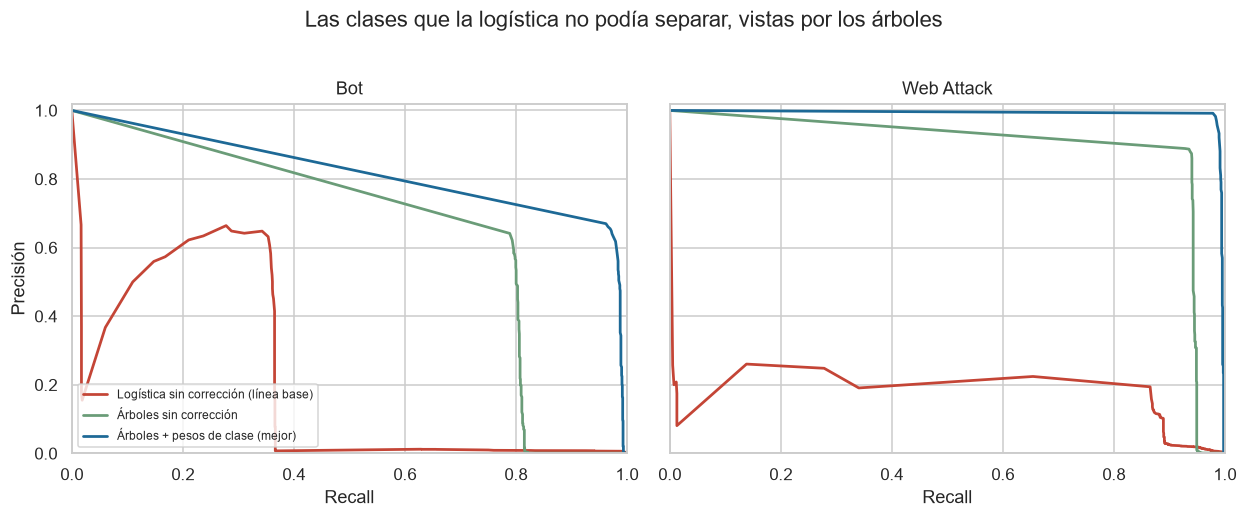
\includegraphics[width=0.86\textwidth]{figures/10_pr_clases_atascadas.png}
\caption{Verificación del supuesto de linealidad. Las curvas se desplazan
hacia la esquina superior derecha al cambiar de familia de modelo, no al
cambiar la técnica de desbalance. Esta es la evidencia de que el supuesto de
separabilidad lineal no se cumple para estas clases.}
\label{fig:atascadas}
\end{figure}

% =====================================================================
\section{Entrenamiento, validación, parametrización y métricas}
% =====================================================================

\subsection{Protocolo experimental}\label{sec:protocolo}

\begin{itemize}
\item \textbf{Partición única:} 80\% entrenamiento (1.998.462 flujos) y 20\%
prueba (499.616), estratificada por clase para preservar las proporciones
incluso en las clases más raras. El conjunto de prueba se apartó una sola vez
y \textbf{no se utilizó} durante todo el desarrollo.
\item \textbf{Validación cruzada estratificada de 5 particiones} sobre el
entrenamiento para la comparación de alternativas, la selección de modelo y
el ajuste del punto de operación. Se reporta media $\pm$ desviación entre
particiones. Una excepción, por costo computacional: la \emph{importancia por
permutación} se midió con una sola partición ---modelo ajustado con el
80\,\% de la primera y medido sobre 300.000 flujos de su validación---
(Cuadro~\ref{tab:param-protocolo}).
\item \textbf{Selección de variables:} 71 $\rightarrow$ 48, decidida
\emph{únicamente} con el conjunto de entrenamiento (Cuadro~\ref{tab:supuestos}; evidencia en el Apéndice~\ref{ap:colinealidad}).
\item \textbf{Control de fuga de información:} deduplicación previa a la
partición; escalado y remuestreo \emph{dentro} del pipeline de validación, de
modo que solo se ajustan con el tramo de entrenamiento de cada partición.
\item \textbf{Reproducibilidad:} semilla fija (42) en todo el proceso y
versiones exactas de dependencias.
\end{itemize}

\noindent\textbf{Parametrización:} El modelo de árboles se configura con un
máximo de 200 iteraciones (\texttt{max\_iter=200}), ponderación balanceada de
clases y semilla 42; el resto de sus parámetros queda en los valores por
defecto de la librería. Con más de 10.000 observaciones, scikit-learn activa
automáticamente la \textbf{parada temprana} (\texttt{early\_stopping='auto'}):
reserva el 10\,\% del tramo de entrenamiento como validación interna y detiene
el entrenamiento cuando la pérdida sobre esa validación deja de mejorar
durante 10 iteraciones seguidas. Por eso 200 es un \emph{techo}, no el número
de iteraciones usadas: el clasificador multiclase final se detuvo en
\textbf{43 iteraciones} (473 árboles, uno por clase y por iteración) y el
binario en \textbf{110}, cifras leídas del atributo \texttt{n\_iter\_} de los
modelos serializados (Apéndice~\ref{ap:parametros}). SMOTE eleva a 20.000
casos las clases con menos de ese umbral (igualarlas a la clase mayoritaria
habría exigido fabricar $\approx$14 millones de filas sintéticas); el
submuestreo reduce la clase benigna a 200.000 casos antes de aplicar SMOTE.

\noindent\textbf{Cómo se fija el umbral del detector de anomalías (cuantiles
del lunes):} El Isolation Forest no produce una etiqueta
sino un \emph{score} de qué tan normal se ve cada flujo; para convertirlo en
una decisión hace falta un corte, y ese corte se fija en cuatro pasos.
(1)~El detector se entrena únicamente con el tráfico del \textbf{lunes}, el
único día de la semana sin ataques (394.236 flujos benignos del conjunto de
entrenamiento), con el escalado ajustado sobre ese mismo tráfico. (2)~Luego
se le pide puntuar ese mismo tráfico conocido-normal, lo que produce una
distribución empírica de los scores de flujos que \emph{sabemos} normales.
(3)~El umbral se fija en un percentil de esa distribución (el 1\,\% como
referencia; 0,5\,\% y 2\,\% como alternativas que el tablero permite elegir),
de modo que, por construcción, exactamente ese porcentaje del tráfico
conocido-normal queda por debajo del corte. (4)~Cualquier flujo de otro día
cuyo score caiga por debajo del corte se marca como anómalo. La ventaja es
que el umbral no es un número arbitrario sino un \textbf{presupuesto
explícito de falsas alarmas}: elegir el 1\,\% significa ``acepto equivocarme
en 1 de cada 100 flujos normales''. El valor numérico del corte (por ejemplo,
$-0{,}614$ al 1\,\%) no tiene significado por sí mismo y por eso no se
reporta como parámetro sino como consecuencia del percentil elegido. Fijarlo
así reconoce además la advertencia de la literatura de que el ``benigno'' del
lunes puede contener ataques sin etiquetar: el percentil asume explícitamente
cierta contaminación en lugar de suponer un lunes perfectamente limpio. Y es
lo que permite medir la deriva (R11): si en otro día la fracción de tráfico
normal que cae bajo el corte se aleja del presupuesto, el tráfico normal
cambió y el detector debe recalibrarse.

\noindent\textbf{Calibración de hiperparámetros:} No se realizó una búsqueda
exhaustiva de hiperparámetros, de forma deliberada. La configuración exacta
con la que se entrenó cada modelo ---qué se fijó explícitamente y qué quedó en
el valor por defecto de la librería, leída de los modelos serializados y del
código, no reconstruida de memoria--- se reporta parámetro por parámetro en
el Apéndice~\ref{ap:parametros}. Con esa configuración el modelo ya superaba
el requerimiento de desempeño por más de tres puntos de macro-F1, y la matriz
de la Sección~\ref{sec:resultados} muestra que la variación atribuible a la
familia de modelo y a la técnica de desbalance (de 0,543 a 0,970) domina
ampliamente cualquier ganancia esperable de un ajuste fino de parámetros. El
esfuerzo de calibración se dirigió, en cambio, donde el análisis mostró
margen real: el \emph{punto de operación} de la clase Bot
(Sección~\ref{sec:ajustes}, ajuste 4), fijado con datos de entrenamiento
exclusivamente. Una búsqueda adicional habría añadido riesgo de sobreajustar
al conjunto de validación a cambio de una ganancia marginal.

\subsection{Justificación de las métricas}

La elección de métricas es clave en problemas con este nivel de desbalance:

\begin{itemize}
\item \textbf{Exactitud (accuracy): descartada.} Con 83\% de tráfico benigno
en el conjunto ya depurado (80,3\% en los datos crudos: la deduplicación
redujo más a los ataques que al tráfico normal), un clasificador que responda
siempre ``normal'' alcanza 83\% de exactitud sin
detectar un solo ataque. Se verificó empíricamente: ese clasificador trivial
obtiene macro-F1 de 0,082 en el problema multiclase.
\item \textbf{Macro-F1: métrica principal.} Promedia el F1 de todas las
clases con igual peso, de modo que una clase con 1.500 casos pesa lo mismo
que una con dos millones. Es la métrica adecuada cuando las clases raras son
las que importan.
\item \textbf{Precisión y recall por clase: obligatorios.} El promedio puede
ocultar que una clase concreta no se detecta. En el contexto del SOC tienen
lectura directa: el recall es la fracción de ataques encontrados; la
precisión, la fracción de alarmas que no son falsas (fatiga de alertas).
\item \textbf{Curvas precision-recall y AP en lugar de ROC/AUC.} La tasa de
falsos positivos que usa la curva ROC tiene por denominador la clase
mayoritaria: con dos millones de flujos benignos, 40.000 falsas alarmas son
apenas un 2\% y la curva luce excelente, mientras la precisión real se
desploma. La curva PR expone ese costo. Además, el AP resultó una herramienta
\emph{de diagnóstico}: un AP alto con recall bajo indica un problema de
umbral, mientras que un AP bajo indica que el modelo no separa la clase.
\item \textbf{Macro-F1 restringido a clases de ataque:} se reporta junto al
global como cifra más exigente, al excluir del promedio la clase benigna.
\end{itemize}

\subsection{Líneas base}

Antes de experimentar se fijaron dos tipos de referencia (baseline) contra los cuales
medir cualquier mejora posterior (Cuadro~\ref{tab:baseline}). La primera es el
\textbf{clasificador trivial}: un modelo que responde siempre la clase
mayoritaria sin mirar los datos. Marca lo que sería el piso absoluto, porque cualquier
modelo que no lo supere no estaría aprendiendo nada. La segunda es la
\textbf{regresión logística sin corrección de desbalance}, que representa la
solución más simple y transparente aplicable al problema. Ambas se calcularon
con el mismo protocolo de validación cruzada que las alternativas posteriores,
de modo que todas las cifras del reporte son comparables entre sí.

\begin{table}[H]
\centering
\caption{Líneas base (validación cruzada sobre el conjunto de entrenamiento).}
\label{tab:baseline}
\small
\begin{tabular}{L{7.5cm} c}
\toprule
\textbf{Configuración de referencia} & \textbf{macro-F1} \\
\midrule
Binaria --- clasificador trivial (siempre ``normal'') & 0,453 \\
Binaria --- regresión logística & 0,921 \\
Multiclase --- clasificador trivial (siempre ``benigno'') & 0,082 \\
Multiclase --- regresión logística & 0,701 \\
\bottomrule
\end{tabular}
\end{table}

% =====================================================================
\section{Análisis de resultados}
\label{sec:resultados}
% =====================================================================

\subsection{Comparación de alternativas}

El Cuadro~\ref{tab:matriz} presenta las ocho combinaciones evaluadas bajo
condiciones idénticas, y la Figura~\ref{fig:matriz} las ordena visualmente.

\begin{table}[H]
\centering
\caption{Matriz de alternativas: macro-F1 (media $\pm$ desviación entre las 5 particiones).}
\label{tab:matriz}
\small
\setlength{\tabcolsep}{4pt}
\begin{tabular}{L{3.6cm} cccc}
\toprule
\textbf{Modelo} & \textbf{Sin corrección} & \textbf{Pesos de clase} & \textbf{SMOTE} & \textbf{Submues.\ + SMOTE} \\
\midrule
Regresión logística & 0,700 $\pm$ 0,014 & 0,543 $\pm$ 0,004 & 0,832 $\pm$ 0,005 & 0,650 $\pm$ 0,002 \\
\textbf{Árboles (HistGB)} & 0,948 $\pm$ 0,008 & \textbf{0,970 $\pm$ 0,002} & 0,966 $\pm$ 0,003 & 0,937 $\pm$ 0,046 \\
\bottomrule
\end{tabular}
\end{table}

\begin{figure}[H]
\centering
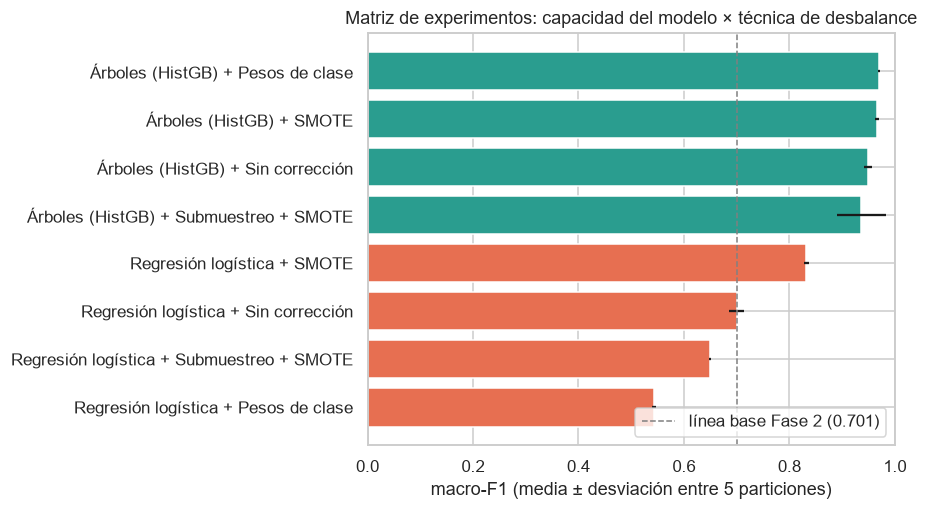
\includegraphics[width=0.80\textwidth]{figures/07_macro_f1_experimentos.png}
\caption{Las ocho combinaciones ordenadas por desempeño. Todas las
configuraciones basadas en árboles superan a todas las lineales.}
\label{fig:matriz}
\end{figure}

\noindent Encontramos tres hallazgos a partir de la matriz:

\begin{enumerate}
\item \textbf{La capacidad del modelo pesó más que la técnica de
desbalance.} La peor configuración de árboles (0,937) supera a la mejor
configuración lineal (0,832). Esto nos indicó que más que ``falta
corrección de desbalance'' era ``falta capacidad de representación''.
\item \textbf{Reponderar sin capacidad es contraproducente.} Los pesos de
clase \emph{hunden} a la regresión logística (0,700 $\rightarrow$ 0,543):
elevan el recall de las clases minoritarias a $\approx$0,99 pero con
precisión de 0,02--0,03, lo que equivale a $\approx$264.000 flujos benignos
marcados como ataque. Con un modelo capaz, la misma técnica es la mejor
(0,948 $\rightarrow$ 0,970).
\item \textbf{La estabilidad importa tanto como la media.} La combinación
submuestreo + SMOTE se descartó no por su media (0,937) sino por su
desviación (0,046): una de las particiones cayó a 0,846.
\end{enumerate}

\subsection{Modelo seleccionado para cada requerimiento}

Con la evidencia anterior se fijó qué modelo responde a cada requerimiento
aprobado del prototipo. Los códigos son los mismos del Cuadro~\ref{tab:req-modelo}, y el enunciado de cada uno se repite aquí para facilitar la lectura.

\begin{itemize}
\item \textbf{R1, R6 y R14} --- clasificar el tipo de ataque pese al
desbalance, con desempeño accionable: \textbf{HistGradientBoosting con pesos
de clase}.
\item \textbf{R3} --- explicar en qué se basa el modelo:
\textbf{importancia por permutación} para la lectura global y \textbf{SHAP}
para la explicación de cada alerta individual. La regresión logística se
conserva como lectura auxiliar del análisis, no como componente del artefacto.
\item \textbf{R4} --- detectar comportamientos anómalos no etiquetados:
\textbf{Isolation Forest} entrenado únicamente con tráfico benigno. El Local
Outlier Factor se documenta como contraste y no se despliega.
\end{itemize}

% =====================================================================
\section{Ajustes implementados a partir de los resultados}
\label{sec:ajustes}
% =====================================================================

El análisis condujo a cinco ajustes, tres de ellos sobre la propia definición
del problema de analítica:

\paragraph{1. Ajuste al esquema de solución: de un modelo a tres.}
Consecuencia directa del hallazgo de linealidad y de la escasez de dos
clases. Ningún modelo único cubre el problema completo
(Figura~\ref{fig:arquitectura}).

\paragraph{2. Ajuste al problema de analítica: agrupación de clases:}
Los tres ataques web (1.470, 652 y 21 casos) se agrupan en la familia
``Web Attack''. La agrupación es la natural del dominio: los tres
atacan la aplicación web.

\paragraph{3. Ajuste al problema de analítica: exclusión honesta de clases:}
Heartbleed (11 casos) e Infiltration (36) se excluyen del problema
multiclase, ya que con validación cruzada de 5 particiones aportarían dos a siete
casos por partición y cualquier métrica por clase sería ruido. Se evalúan en
el nivel binario y con el detector de anomalías, y se reportan siempre
acompañadas de su tamaño de muestra. Declarar la limitación es preferible a
publicar una cifra que el dato realmente no sostiene.

\paragraph{4. Ajuste al punto de operación: umbral para la clase Bot.}
La clase Bot alcanzaba precisión de 0,614 con recall de 0,980, es decir cuatro de cada
diez alarmas eran falsas. Su AP de 0,91 indicaba margen para intercambiar
recall por precisión. Se fijó, \emph{con datos de entrenamiento
exclusivamente}, la regla de emitir la alarma de Bot solo cuando la probabilidad
supere 0,999. Resultado sobre el conjunto de prueba: precisión 0,947 con
recall 0,728.

\paragraph{5. Verificación de validez: la prueba del puerto de destino.}
La segunda variable más influyente resultó ser el puerto del servicio
contactado, un \emph{identificador} y no un comportamiento: en el conjunto de
datos cada ataque usa siempre su puerto canónico, algo que en una red real no necesariamente tiene que pasar. Se reentrenó el modelo sin esa variable
(Figura~\ref{fig:puerto}): el desempeño pasó de 0,970 a 0,950 en validación
cruzada y de 0,967 a 0,942 en prueba. La caída es pequeña y el recall se
mantiene en todas las clases, lo que indica que el modelo aprende
comportamiento, y el costo se concentra en la precisión de las dos clases
difíciles. Por honestidad metodológica, ambas cifras se reportan juntas y la
variante sin puerto se declara como la \textbf{estimación conservadora}.

\begin{figure}[H]
\centering
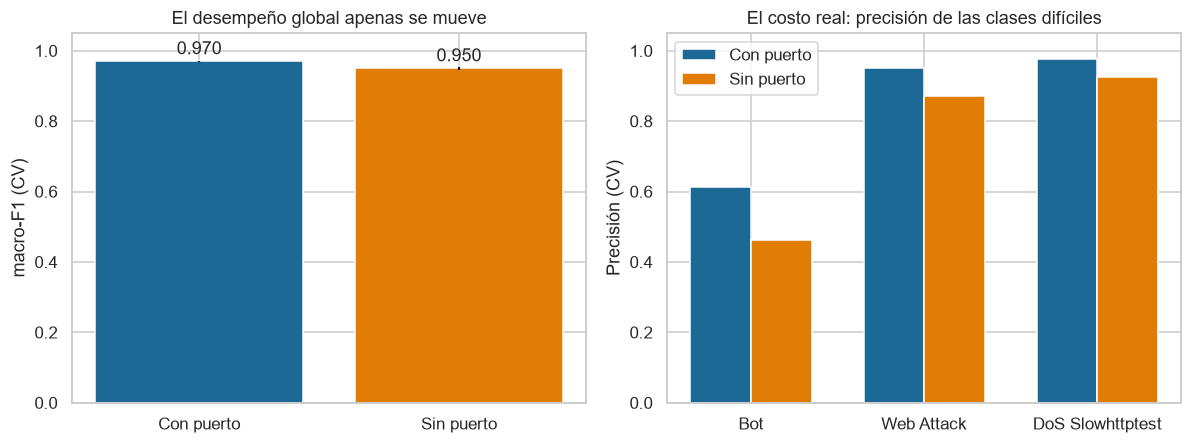
\includegraphics[width=0.86\textwidth]{figures/13_experimento_puerto.png}
\caption{Prueba del puerto de destino. El desempeño global apenas se mueve al
retirar el identificador; el costo se localiza en la precisión de las clases
difíciles.}
\label{fig:puerto}
\end{figure}

\subsection{Resultados sobre el conjunto de prueba}

Con el modelo ya definido, se utilizó el conjunto de prueba por primera y
única vez (para tener los resultados como una medición completamente limpia).

\begin{table}[H]
\centering
\caption{Evaluación final sobre el conjunto de prueba (499.616 flujos).}
\label{tab:test}
\small
\begin{tabular}{L{8.2cm} c c}
\toprule
\textbf{Configuración} & \textbf{macro-F1} & \textbf{Solo ataques} \\
\midrule
\textbf{Modelo final} (con puerto + umbral de Bot) & \textbf{0,975} & \textbf{0,972} \\
Con puerto, regla estándar & 0,967 & 0,964 \\
\textbf{Estimación conservadora} (sin el puerto) & \textbf{0,942} & \textbf{0,937} \\
\bottomrule
\end{tabular}
\end{table}

\noindent\textbf{Validez del protocolo:} Las cifras de prueba coinciden con
las de validación cruzada (0,970 $\pm$ 0,002 frente a 0,967 con puerto;
0,950 $\pm$ 0,004 frente a 0,942 sin él). Esa coincidencia es la evidencia de
que no hubo sobreajuste ni fuga de información.

\noindent\textbf{Cumplimiento de requerimientos:} R6 exigía macro-F1
$\geq$ 0,94: se obtuvo 0,975 (0,942 en la estimación conservadora). R2 exigía
falsas alarmas $\leq$ 0,2\% sobre tráfico benigno: se obtuvo 0,12\%. R5
exigía superar sustancialmente el clasificador trivial: 0,975 frente a 0,082.
La segunda parte de R5, la reducción de la carga de revisión, se materializa
en el panel de resumen del tablero, que la calcula sobre el archivo que carga
el usuario.

\noindent\textbf{Detección no supervisada (R4):} El Isolation Forest,
entrenado únicamente con tráfico benigno, detecta 89\% de los flujos de
Heartbleed, 52\% de DoS slowloris y 48\% de Infiltration (Heartbleed e
Infiltration son justamente las familias que el modelo supervisado no pudo
aprender) con un presupuesto de
1\% de falsas alarmas (umbral por cuantiles del lunes, Sección~\ref{sec:protocolo}). Su recall global es de 11,8\%, y se documenta
explícitamente su punto ciego: es incapaz de detectar ataques camuflados
(fuerza bruta, escaneo de puertos, botnet), porque en ellos cada flujo
individual parece normal y lo anómalo reside precisamente en el agregado. El recall
superior a 0,4 en las familias estructuralmente raras se cumple como exigía el R4

\noindent\textbf{Deriva temporal (R11):} La tasa de falsas alarmas del
detector se mantuvo en torno al 1\% previsto casi todos los días, con una
excepción documentada: un tramo del viernes alcanzó 9,6\%. Se reporta como
señal de que un despliegue real exigiría recalibración periódica.

% =====================================================================
\section{Estado de implementación y plan para completar el prototipo}
\label{sec:plan}
% =====================================================================

\subsection{Componentes ya implementados}

A la fecha de este reporte están implementados y verificados:

\begin{itemize}
\item \textbf{Modelos serializados} (1,3\,MB en total) con sus metadatos, y
verificación de determinismo: los umbrales reproducidos coinciden decimal a
decimal con los del análisis.
\item \textbf{Tablero web} (Streamlit) con seis pantallas funcionales:
resumen, clasificación, detección de anomalías, interpretabilidad, cola de
alertas y reportes. Incluye validación de archivos de entrada, filtros,
exportación en CSV e historial de sesión. La interfaz se seguirá refinando
antes de la entrega final.
\item \textbf{Archivos de demostración}: dos muestras del conjunto de prueba.
Una con 499 flujos con 39,9\,\% de ataque y la otra con 500 flujos con 5,0\,\%, esta última tiene una proporción más realista, y se crearon para probar la herramienta con archivos mucho más manejables.
\item \textbf{Pruebas automatizadas} (25 casos) sobre validación de entradas,
clasificación, umbrales y explicaciones. Los scripts se ejecutan fuera del
repositorio, incorporarlos a él está pendiente.
\item \textbf{Verificación de desempeño (R9):} 50.000 flujos clasificados en
menos de un segundo (0,7--0,8\,s en mediciones repetidas) con un pico de
memoria cercano a 390\,MB, frente a la promesa de 30 segundos y 1\,GB
disponible.
\item \textbf{Licencias:} todas las dependencias son de código abierto
con licencias permisivas (BSD, MIT, Apache 2.0, PSF), compatibles con uso
académico.
\end{itemize}

\subsection{Componentes pendientes y plan}

El Cuadro~\ref{tab:plan} lista los componentes que restan, con el
requerimiento que los motiva. Todos ellos se completan como parte de la
entrega final del proyecto, antes de la evaluación del prototipo y de la
presentación ejecutiva.

\begin{table}[H]
\centering
\caption{Plan para completar la implementación del prototipo.}
\label{tab:plan}
\footnotesize\setlength{\tabcolsep}{4pt}
\begin{tabular}{L{4.2cm} L{7.4cm} L{2.2cm}}
\toprule
\textbf{Pendiente} & \textbf{Descripción} & \textbf{Req.} \\
\midrule
Despliegue en URL pública & Publicar el tablero en alojamiento gratuito con la versión de Python con la que se congeló el entorno; verificar el tiempo de reanudación tras inactividad & R10, R22 \\
Manual de usuario & Qué hace la herramienta, sus limitaciones y advertencias, requisitos previos y al menos tres casos de uso paso a paso & Entregable \\
Rúbrica de pruebas diligenciada & Tabla de requerimientos con evidencia de cumplimiento, ajustes implementados y justificación de lo no satisfecho & Entregable \\
Tabla de falsas alarmas por día en el tablero & Los datos ya están calculados; falta exponerlos en la interfaz & R11 \\
Prueba de usabilidad con usuario ajeno & Verificar que un usuario ajeno completa cargar $\rightarrow$ revisar $\rightarrow$ exportar sin asistencia & R20 \\
Scripts de prueba en el repositorio & Los 25 casos automatizados se ejecutan hoy fuera del repositorio; incorporarlos los hace verificables por un tercero & Entregable \\
Presentación ejecutiva & Siete minutos: problema, esquema de solución, demostración y propuesta de valor & Entregable \\
\bottomrule
\end{tabular}
\end{table}

\subsection{Riesgos identificados}

\begin{itemize}
\item \textbf{Sensibilidad de versión de los artefactos:} Los modelos
serializados dependen de la versión exacta de la librería con que se
generaron. Mitigación: versiones congeladas, verificación al arrancar y
mensaje de advertencia explícito.
\item \textbf{Limitaciones del alojamiento gratuito:} No garantiza
persistencia entre reinicios ni tiempos de reanudación acotados. Mitigación:
el historial se declara como de sesión, no persistente.
\item \textbf{Calidad del conjunto de datos:} Encontramos papers que documentan errores
de etiquetado en CIC-IDS2017 (Engelen et al., 2021; Rosay et al., 2022;
Lanvin et al., 2023). Se declara como limitación y afecta
principalmente al detector no supervisado, y se mitiga fijando el umbral por
cuantiles asumiendo explícitamente cierta contaminación.
\end{itemize}

% =====================================================================
\section{Conclusiones}
% =====================================================================

\begin{enumerate}
\item El tipo de ataque puede clasificarse con alta calidad pese al
desbalance extremo: macro-F1 de 0,975 sobre el conjunto de prueba, y 0,942 en
la estimación conservadora que no depende del puerto de destino.
\item \textbf{El diagnóstico correcto importa más que la técnica.} Las clases
que parecían imposibles no necesitaban más remuestreo sino un modelo capaz de
representar fronteras no lineales. Reponderar sin capacidad multiplica las
falsas alarmas.
\item Los ataques se distinguen por \emph{comportamiento} (duración,
ritmo entre paquetes, tamaños) y no solo por el puerto: retirar el único
identificador cuesta entre dos y tres puntos de macro-F1.
\item El modelo no supervisado es un complemento, no un sustituto: detecta
sin etiquetas justamente las familias que el supervisado no puede aprender,
pero es ciego a los ataques camuflados.
\item El prototipo está implementado y verificado en sus componentes
centrales; el plan de la Sección~\ref{sec:plan} cierra lo pendiente antes de la evaluación
y la presentación ejecutiva.
\end{enumerate}

% =====================================================================
\section*{Referencias}
\addcontentsline{toc}{section}{Referencias}
% =====================================================================

\begin{itemize}[leftmargin=*, label={}]
\item Sharafaldin, I., Lashkari, A. H., \& Ghorbani, A. A. (2018).
\emph{Toward Generating a New Intrusion Detection Dataset and Intrusion
Traffic Characterization}. 4th International Conference on Information
Systems Security and Privacy (ICISSP), Portugal, enero de 2018.
\item Engelen, G., Rimmer, V., \& Joosen, W. (2021). \emph{Troubleshooting an
Intrusion Detection Dataset: the CICIDS2017 Case Study}. IEEE Security and
Privacy Workshops.
\item Rosay, A., et al. (2022). \emph{Network Intrusion Detection: A
Comprehensive Analysis of CIC-IDS2017}. ICISSP.
\item Lanvin, M., et al. (2023). \emph{Errors in the CICIDS2017 Dataset and
the Significant Differences in Detection Performances It Makes}. CRiSIS 2022.
\item Lundberg, S. M., \& Lee, S. I. (2017). \emph{A Unified Approach to
Interpreting Model Predictions}. Advances in Neural Information Processing
Systems (NeurIPS).
\end{itemize}

% =====================================================================
\clearpage
\appendix
% Cuadros y figuras de los apéndices se numeran A.1, B.1, ... para
% distinguirlos de los del cuerpo del reporte.
\renewcommand{\thetable}{\Alph{section}.\arabic{table}}
\renewcommand{\thefigure}{\Alph{section}.\arabic{figure}}
\setcounter{table}{0}\setcounter{figure}{0}
\section{Evidencia de colinealidad: los 13 bloques de variables redundantes}
\label{ap:colinealidad}
% =====================================================================

La retroalimentación pidió anexar una lista o mapa de correlaciones que
respalde la poda de 71 a 48 variables (Cuadro~\ref{tab:supuestos}). Este
apéndice la reproduce sobre los mismos datos con los que se tomó la decisión.

\paragraph{Cómo se calculó.} Sobre una muestra de 500.000 flujos del
\textbf{conjunto de entrenamiento} (semilla 42; el conjunto de prueba no
participa) se calculó la correlación de Pearson en valor absoluto entre las 71
variables numéricas del dataset depurado. Hay \textbf{45 pares} con
$|r| > 0{,}95$. Si cada variable es un nodo y cada par por encima del umbral
es un arco, esos 45 pares forman \textbf{13 componentes conexas}: los
\emph{bloques} del Cuadro~\ref{tab:bloques}, que abarcan 36 variables. De
cada bloque se conserva \textbf{una representante}, elegida por
interpretabilidad (el nombre más directo de explicar a un lector no experto
en redes), y se eliminan las otras 23: $71 - 23 = 48$. La razón de la poda es
que dos columnas casi idénticas se reparten la importancia en los modelos y
ensucian la interpretación; para la regresión logística, además, violan el
supuesto de baja colinealidad.

\paragraph{Cómo leer la figura.} La Figura~\ref{fig:bloques} muestra el mapa
de $|r|$ entre las 36 variables implicadas, ordenadas bloque a bloque
(representante primero, marcada con $\star$), con cada bloque recuadrado y
los valores anotados dentro de él. Dos precisiones: (i)~un bloque es una
componente conexa, así que dos variables del mismo bloque no tienen por qué
superar 0,95 \emph{entre sí} ---por ejemplo, \texttt{Bwd Packet Length Mean} y
\texttt{Bwd Packet Length Std} correlacionan 0,94, pero ambas superan 0,95 con
\texttt{Bwd Packet Length Max}---; (ii)~fuera de los recuadros hay
correlaciones altas pero por debajo del umbral (tonos medios), que
deliberadamente no motivaron eliminaciones. La figura del análisis
exploratorio (\texttt{02\_correlaciones\_redundantes.png}) usaba $|r| > 0{,}999$
sobre una muestra del dataset completo y servía para ilustrar los alias
exactos; la de este apéndice se calcula al umbral con el que realmente se
decidió y solo sobre el entrenamiento, y coincide exactamente con el cuadro.

\begin{figure}[H]
\centering
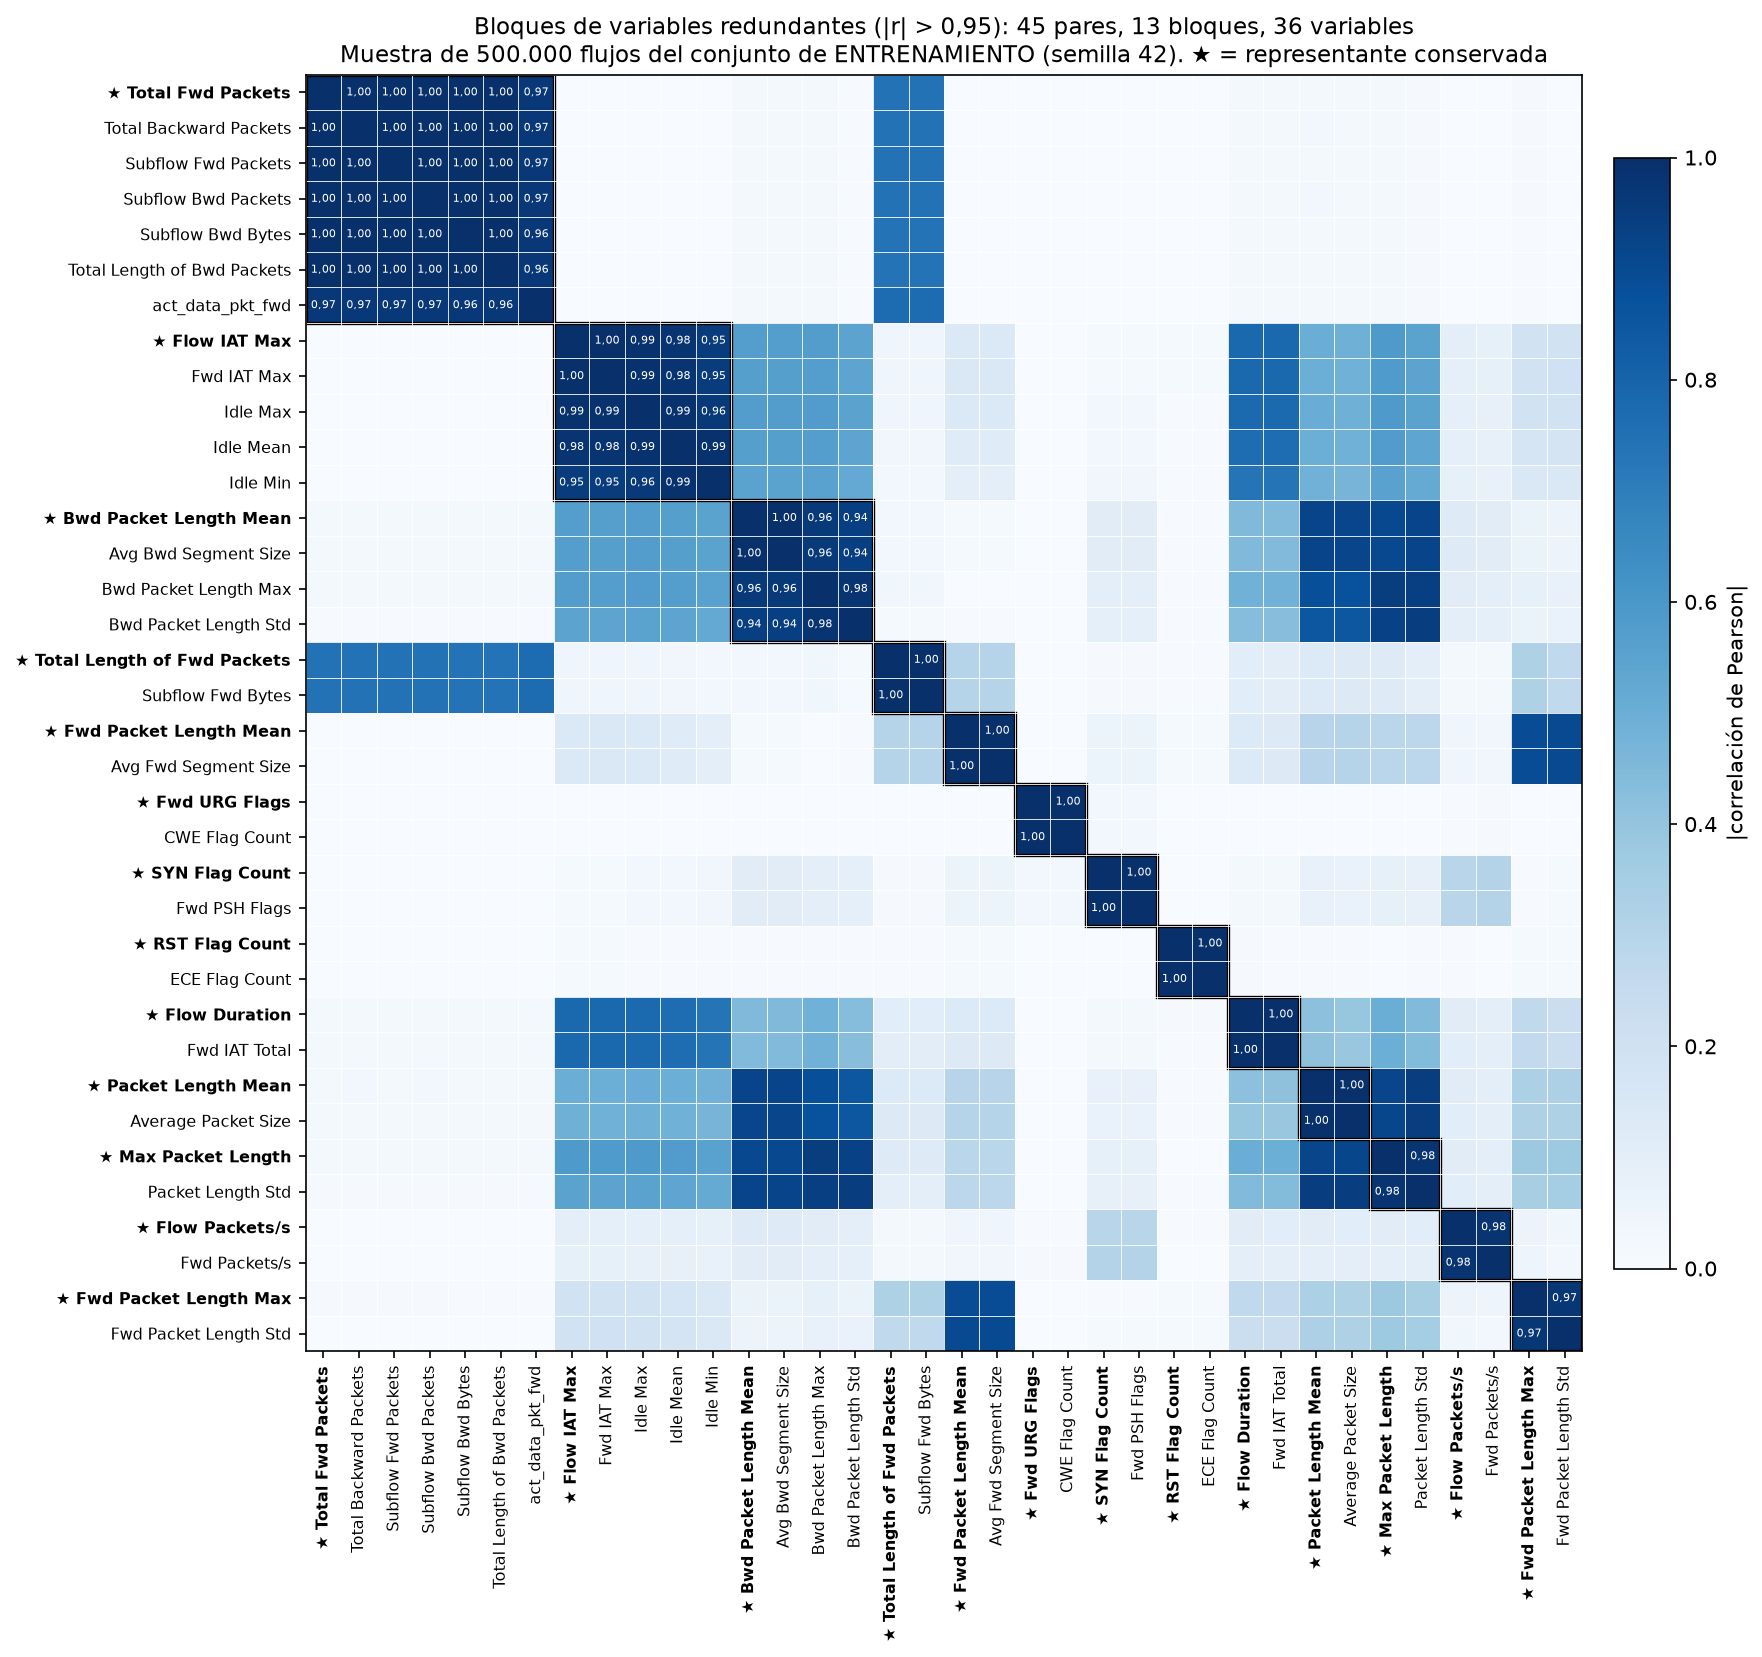
\includegraphics[width=\textwidth]{figures/18_correlaciones_train_095.png}
\caption{Mapa de $|r|$ (correlación de Pearson en valor absoluto) entre las 36
variables que participan en algún par con $|r| > 0{,}95$, sobre 500.000 flujos
del conjunto de entrenamiento (semilla 42). Cada recuadro negro es uno de los
13 bloques del Cuadro~\ref{tab:bloques}; $\star$ marca la representante
conservada. Los valores anotados son los de cada bloque; fuera de los
recuadros ninguna pareja supera el umbral.}
\label{fig:bloques}
\end{figure}

\paragraph{Reproducibilidad.} Los bloques se re-derivan con
\texttt{calcular\_grupos()} en \texttt{src/features.py} y el script
\texttt{reports/apendices/generar\_apendices.py} verifica que coinciden uno a
uno con la lista \texttt{GRUPOS\_CORRELACIONADOS} antes de dibujar la figura y
escribir el cuadro; el detalle numérico por bloque queda en
\texttt{reports/apendices/bloques\_correlacion\_train.csv}.

{\footnotesize
% Generado por reports/apendices/generar_apendices.py a partir de
% GRUPOS_CORRELACIONADOS (src/features.py). No editar a mano.
\begin{longtable}{C{0.6cm} L{3.0cm} L{4.2cm} L{6.3cm}}
\caption{Los 13 bloques de variables redundantes ($|r| > 0{,}95$ sobre 500.000 flujos del conjunto de entrenamiento, semilla 42). Texto tomado literalmente de \texttt{GRUPOS\_CORRELACIONADOS} en \texttt{src/features.py}.}\label{tab:bloques}\\
\toprule
\textbf{\#} & \textbf{Representante conservada} & \textbf{Variables eliminadas} & \textbf{Razón de la elección} \\
\midrule
\endfirsthead
\toprule
\textbf{\#} & \textbf{Representante conservada} & \textbf{Variables eliminadas} & \textbf{Razón de la elección} \\
\midrule
\endhead
\bottomrule
\endfoot
1 & \texttt{Total Fwd Packets} & \texttt{Total Backward Packets}, \texttt{Subflow Fwd Packets}, \texttt{Subflow Bwd Packets}, \texttt{Subflow Bwd Bytes}, \texttt{Total Length of Bwd Packets}, \texttt{act\_data\_pkt\_fwd} & Todas cuentan volumen de la conversación y se mueven juntas; 'paquetes enviados por el origen' es el conteo más directo. Las 'Subflow *' son alias exactos de los totales. \\
2 & \texttt{Flow IAT Max} & \texttt{Fwd IAT Max}, \texttt{Idle Max}, \texttt{Idle Mean}, \texttt{Idle Min} & Todas capturan el mayor silencio dentro de la conversación; 'Flow IAT Max' es la versión global. \\
3 & \texttt{Bwd Packet Length Mean} & \texttt{Avg Bwd Segment Size}, \texttt{Bwd Packet Length Max}, \texttt{Bwd Packet Length Std} & Tamaño de los paquetes de respuesta; 'Avg Bwd Segment Size' es un alias exacto de la media, y máximo/desviación van casi pegados a ella. \\
4 & \texttt{Total Length of Fwd Packets} & \texttt{Subflow Fwd Bytes} & Alias exacto (r=1.000); se conserva el nombre directo: bytes enviados por el origen. \\
5 & \texttt{Fwd Packet Length Mean} & \texttt{Avg Fwd Segment Size} & Alias exacto (r=1.000) del tamaño medio de paquete de ida. \\
6 & \texttt{Fwd URG Flags} & \texttt{CWE Flag Count} & Idénticas en los datos (r=1.000); se conserva la bandera TCP estándar (URG), mejor documentada que el conteo 'CWE'. \\
7 & \texttt{SYN Flag Count} & \texttt{Fwd PSH Flags} & Idénticas en los datos (r=1.000); SYN (inicio de conexión) es clave para explicar escaneos de puertos. \\
8 & \texttt{RST Flag Count} & \texttt{ECE Flag Count} & Idénticas en los datos (r=1.000); RST (conexión rechazada/cortada) es la más interpretable. \\
9 & \texttt{Flow Duration} & \texttt{Fwd IAT Total} & r=0.999; la duración de la conversación es la feature más fácil de explicar del dataset. \\
10 & \texttt{Packet Length Mean} & \texttt{Average Packet Size} & r=0.998; son dos fórmulas casi iguales del tamaño medio de paquete. \\
11 & \texttt{Max Packet Length} & \texttt{Packet Length Std} & r=0.984; el máximo es más directo de explicar que la desviación. \\
12 & \texttt{Flow Packets/s} & \texttt{Fwd Packets/s} & r=0.983; se conserva el ritmo global de la conversación. \\
13 & \texttt{Fwd Packet Length Max} & \texttt{Fwd Packet Length Std} & r=0.969; mismo criterio: máximo antes que desviación. \\
\end{longtable}
}

% =====================================================================
\section{Configuración de parámetros}
\label{ap:parametros}
\setcounter{table}{0}\setcounter{figure}{0}
% =====================================================================

La retroalimentación pidió reportar la configuración de los parámetros en
lugar de decir que se usaron ``valores estándar''. Nada de lo que sigue se
escribió de memoria: las tablas de los modelos desplegados se generaron
leyendo \texttt{get\_params()} y los atributos ajustados de los archivos de
\texttt{models/}; las del protocolo, instanciando los estimadores con la misma
función del código que los construyó en los experimentos
(\texttt{construir\_pipeline} en \texttt{src/experimentos.py}) y leyendo las
constantes de \texttt{src/}. El script que lo hace es
\texttt{reports/apendices/generar\_apendices.py}; su salida tabular completa
(264 filas) está en \texttt{reports/apendices/parametros\_modelos.csv}.

\textbf{Qué significa ``explícito''.} Un parámetro se marca como explícito
cuando está \emph{escrito en la llamada del código fuente} (el script lee las
llamadas de \texttt{src/} con el analizador sintáctico de Python y las registra
en \texttt{llamadas\_en\_codigo.csv}), aunque el valor escrito coincida con el
valor por defecto de la librería: es el caso de \texttt{n\_neighbors=20} en el
Local Outlier Factor, de \texttt{n\_splits=5} en la validación cruzada y de
\texttt{n\_repeats=5} en la importancia por permutación, que se señalan como
``explícito (igual al defecto)''. ``Por defecto'' significa que el código no
lo escribe y rige el valor de la librería.

\subsection{Iteraciones reales y parada temprana}

Es el punto donde la lectura del código corrige al documento anterior, que
decía que el modelo de árboles ``usa 200 iteraciones''. En realidad
\texttt{max\_iter=200} es un \textbf{máximo}. \texttt{HistGradientBoosting}
trae \texttt{early\_stopping='auto'}, que se activa cuando hay más de 10.000
observaciones ---siempre, en este proyecto---: reserva el 10\,\% del tramo de
entrenamiento (\texttt{validation\_fraction=0.1}) como validación interna,
ajusta los árboles con el 90\,\% restante y se detiene cuando la pérdida en esa
validación no mejora en más de \texttt{tol}~$=10^{-7}$ durante
\texttt{n\_iter\_no\_change}~$=10$ iteraciones seguidas. El
Cuadro~\ref{tab:iteraciones} resume lo que ocurrió con los modelos
serializados (entrenados con todo el conjunto de entrenamiento, los mismos que
usa el tablero). Los modelos de cada partición de la validación cruzada no se
conservaron (solo sus métricas), por lo que su número exacto de iteraciones no
se reporta; usaron la misma configuración y el mismo techo.

\begin{table}[H]
\centering
\caption{Iteraciones realmente usadas por los modelos serializados, leídas del
atributo \texttt{n\_iter\_}. ``Mejor iteración'' es la de menor pérdida en la
validación interna; el entrenamiento se detuvo 10 iteraciones después.}
\label{tab:iteraciones}
\footnotesize
\begin{tabular}{L{3.4cm} C{1.2cm} C{1.8cm} C{2.0cm} C{1.8cm} C{2.8cm}}
\toprule
\textbf{Modelo} & \textbf{Techo} & \textbf{Parada temprana} & \textbf{Iteraciones usadas} & \textbf{Mejor iteración} & \textbf{Árboles} \\
\midrule
Clasificador multiclase & 200 & activa & \textbf{43} & 33 & 473 (11 por iteración) \\
Clasificador binario & 200 & activa & \textbf{110} & 100 & 110 \\
\bottomrule
\end{tabular}
\end{table}

\subsection{Modelos desplegados (leídos de \texttt{models/})}

Los dos cuadros siguientes listan \emph{todos} los parámetros de los objetos
serializados. Los dos clasificadores comparten exactamente la misma
configuración (se verifica por código), así que van en un solo cuadro con los
atributos ajustados de cada uno en columnas. Los únicos parámetros escritos en
el código son: en los clasificadores, \texttt{class\_weight='balanced'},
\texttt{max\_iter=200} y \texttt{random\_state=42}; en el Isolation Forest,
\texttt{n\_estimators=200}, \texttt{random\_state=42} y \texttt{n\_jobs=-1}
(este último solo reparte el cómputo entre núcleos; no cambia el resultado).
En el Isolation Forest, \texttt{contamination='auto'} queda en su valor por
defecto porque \emph{no se usa}: el corte lo fija el percentil de los scores
del lunes (Sección~\ref{sec:protocolo}); y \texttt{max\_samples='auto'}
significa 256 flujos por árbol, el valor que la librería fija para ese modo.
% Generado por reports/apendices/generar_apendices.py.
Los dos \texttt{StandardScaler} del proyecto ---el del detector, serializado en \texttt{models/}, y el que precede a la regresión logística dentro de cada partición--- se instancian sin argumentos y quedan enteramente por defecto (\texttt{copy=True}, \texttt{with\_mean=True}, \texttt{with\_std=True}). El del detector se ajustó con los 394.236 flujos benignos del lunes (\texttt{n\_samples\_seen\_}) y 48 variables.

{\footnotesize\renewcommand{\arraystretch}{1.05}
% Generado por reports/apendices/generar_apendices.py con get_params() sobre Clasificadores multiclase y binario (misma configuración).
\begin{longtable}{L{3.9cm} L{3.7cm} L{3.0cm} L{2.4cm}}
\caption{Clasificadores multiclase y binario (misma configuración): \texttt{HistGradientBoostingClassifier}, 21 parámetros. En \textbf{negrilla}, los escritos en la llamada del código (aunque coincidan con el valor por defecto); el resto quedó en el valor por defecto de scikit-learn 1.9.0.}\label{tab:param-hgb}\\
\toprule
\textbf{Parámetro} & \textbf{Valor usado} & \textbf{Valor por defecto} & \textbf{Origen} \\
\midrule
\endfirsthead
\toprule
\textbf{Parámetro} & \textbf{Valor usado} & \textbf{Valor por defecto} & \textbf{Origen} \\
\midrule
\endhead
\bottomrule
\endfoot
\texttt{categorical\_features} & \texttt{'from\_dtype'} & \texttt{'from\_dtype'} & por defecto \\
\textbf{\texttt{class\_weight}} & \textbf{\texttt{'balanced'}} & \texttt{None} & explícito \\
\texttt{early\_stopping} & \texttt{'auto'} & \texttt{'auto'} & por defecto \\
\texttt{interaction\_cst} & \texttt{None} & \texttt{None} & por defecto \\
\texttt{l2\_regularization} & \texttt{0.0} & \texttt{0.0} & por defecto \\
\texttt{learning\_rate} & \texttt{0.1} & \texttt{0.1} & por defecto \\
\texttt{loss} & \texttt{'log\_loss'} & \texttt{'log\_loss'} & por defecto \\
\texttt{max\_bins} & \texttt{255} & \texttt{255} & por defecto \\
\texttt{max\_depth} & \texttt{None} & \texttt{None} & por defecto \\
\texttt{max\_features} & \texttt{1.0} & \texttt{1.0} & por defecto \\
\textbf{\texttt{max\_iter}} & \textbf{\texttt{200}} & \texttt{100} & explícito \\
\texttt{max\_leaf\_nodes} & \texttt{31} & \texttt{31} & por defecto \\
\texttt{min\_samples\_leaf} & \texttt{20} & \texttt{20} & por defecto \\
\texttt{monotonic\_cst} & \texttt{None} & \texttt{None} & por defecto \\
\texttt{n\_iter\_no\_change} & \texttt{10} & \texttt{10} & por defecto \\
\textbf{\texttt{random\_state}} & \textbf{\texttt{42}} & \texttt{None} & explícito \\
\texttt{scoring} & \texttt{'loss'} & \texttt{'loss'} & por defecto \\
\texttt{tol} & \texttt{1e-07} & \texttt{1e-07} & por defecto \\
\texttt{validation\_fraction} & \texttt{0.1} & \texttt{0.1} & por defecto \\
\texttt{verbose} & \texttt{0} & \texttt{0} & por defecto \\
\texttt{warm\_start} & \texttt{False} & \texttt{False} & por defecto \\
\midrule
\emph{Atributos ajustados} & \textbf{Multiclase} & \textbf{Binario} & \\
\texttt{do\_early\_stopping\_} & \texttt{True} & \texttt{True} & \\
\texttt{n\_iter\_ (iteraciones realmente usadas)} & \texttt{43} & \texttt{110} & \\
\texttt{n\_trees\_per\_iteration\_} & \texttt{11} & \texttt{1} & \\
\texttt{árboles totales} & \texttt{473} & \texttt{110} & \\
\texttt{mejor iteración en la validación interna} & \texttt{33} & \texttt{100} & \\
\texttt{n\_features\_in\_} & \texttt{48} & \texttt{48} & \\
\texttt{clases} & \texttt{11} & \texttt{2} & \\
\end{longtable}

% Generado por reports/apendices/generar_apendices.py con get_params() sobre Detector de anomalías: bosque.
\begin{longtable}{L{3.9cm} L{3.7cm} L{3.0cm} L{2.4cm}}
\caption{Detector de anomalías: bosque: \texttt{IsolationForest}, 9 parámetros. En \textbf{negrilla}, los escritos en la llamada del código (aunque coincidan con el valor por defecto); el resto quedó en el valor por defecto de scikit-learn 1.9.0.}\label{tab:param-if}\\
\toprule
\textbf{Parámetro} & \textbf{Valor usado} & \textbf{Valor por defecto} & \textbf{Origen} \\
\midrule
\endfirsthead
\toprule
\textbf{Parámetro} & \textbf{Valor usado} & \textbf{Valor por defecto} & \textbf{Origen} \\
\midrule
\endhead
\bottomrule
\endfoot
\texttt{bootstrap} & \texttt{False} & \texttt{False} & por defecto \\
\texttt{contamination} & \texttt{'auto'} & \texttt{'auto'} & por defecto \\
\texttt{max\_features} & \texttt{1.0} & \texttt{1.0} & por defecto \\
\texttt{max\_samples} & \texttt{'auto'} & \texttt{'auto'} & por defecto \\
\textbf{\texttt{n\_estimators}} & \textbf{\texttt{200}} & \texttt{100} & explícito \\
\textbf{\texttt{n\_jobs}} & \textbf{\texttt{-1}} & \texttt{None} & explícito \\
\textbf{\texttt{random\_state}} & \textbf{\texttt{42}} & \texttt{None} & explícito \\
\texttt{verbose} & \texttt{0} & \texttt{0} & por defecto \\
\texttt{warm\_start} & \texttt{False} & \texttt{False} & por defecto \\
\midrule
\multicolumn{4}{l}{\emph{Atributos ajustados (leídos del modelo entrenado)}} \\
\texttt{max\_samples\_ (flujos por árbol)} & \multicolumn{3}{l}{\texttt{256}} \\
\texttt{n\_features\_in\_} & \multicolumn{3}{l}{\texttt{48}} \\
\texttt{umbral cuantil 0,5 \% / 1 \% / 2 \%} & \multicolumn{3}{l}{\texttt{-0,6369 / -0,6140 / -0,5870}} \\
\end{longtable}
}

\subsection{Estimadores del protocolo que no se despliegan}

La regresión logística (referencia lineal), las dos técnicas de remuestreo y
el Local Outlier Factor no viven en \texttt{models/}. Sus parámetros se leen
instanciándolos con el mismo código que los usó. Dos precisiones. En la
regresión logística y en el HistGradientBoosting de la matriz de la Fase 3,
\texttt{class\_weight} está escrito en la llamada (\texttt{class\_weight=peso})
y vale \texttt{None} salvo en la columna ``pesos de clase'', donde vale
\texttt{'balanced'}: por eso figura como explícito aunque en tres de las cuatro
columnas su valor sea el por defecto. Y en la regresión logística,
\texttt{penalty} aparece como \texttt{'deprecated'} porque scikit-learn 1.8
retiró ese parámetro; la regularización efectiva es L2
(\texttt{l1\_ratio=0.0}) con \texttt{C=1.0} y el solucionador \texttt{lbfgs},
todo por defecto.

{\footnotesize\renewcommand{\arraystretch}{1.0}
% Generado por reports/apendices/generar_apendices.py con get_params() sobre Regresión logística (referencia lineal).
\begin{longtable}{L{3.9cm} L{3.7cm} L{3.0cm} L{2.4cm}}
\caption{Regresión logística (referencia lineal): \texttt{LogisticRegression}, 14 parámetros. En \textbf{negrilla}, los escritos en la llamada del código (aunque coincidan con el valor por defecto); el resto quedó en el valor por defecto de scikit-learn 1.9.0.}\label{tab:param-reglog}\\
\toprule
\textbf{Parámetro} & \textbf{Valor usado} & \textbf{Valor por defecto} & \textbf{Origen} \\
\midrule
\endfirsthead
\toprule
\textbf{Parámetro} & \textbf{Valor usado} & \textbf{Valor por defecto} & \textbf{Origen} \\
\midrule
\endhead
\bottomrule
\endfoot
\texttt{C} & \texttt{1.0} & \texttt{1.0} & por defecto \\
\textbf{\texttt{class\_weight}} & \textbf{\texttt{None} $\mid$ \texttt{'balanced'} (columna ``pesos'')} & \texttt{None} & explícito (según la técnica) \\
\texttt{dual} & \texttt{False} & \texttt{False} & por defecto \\
\texttt{fit\_intercept} & \texttt{True} & \texttt{True} & por defecto \\
\texttt{intercept\_scaling} & \texttt{1} & \texttt{1} & por defecto \\
\texttt{l1\_ratio} & \texttt{0.0} & \texttt{0.0} & por defecto \\
\textbf{\texttt{max\_iter}} & \textbf{\texttt{1000}} & \texttt{100} & explícito \\
\texttt{n\_jobs} & \texttt{None} & \texttt{None} & por defecto \\
\texttt{penalty} & \texttt{'deprecated'} & \texttt{'deprecated'} & por defecto \\
\textbf{\texttt{random\_state}} & \textbf{\texttt{42}} & \texttt{None} & explícito \\
\texttt{solver} & \texttt{'lbfgs'} & \texttt{'lbfgs'} & por defecto \\
\texttt{tol} & \texttt{0.0001} & \texttt{0.0001} & por defecto \\
\texttt{verbose} & \texttt{0} & \texttt{0} & por defecto \\
\texttt{warm\_start} & \texttt{False} & \texttt{False} & por defecto \\
\end{longtable}

% Generado por reports/apendices/generar_apendices.py con get_params() sobre SMOTE (\texttt{sampling\_strategy} es la función \texttt{estrategia\_smote}: eleva a 20.000 las clases con menos casos que eso).
\begin{longtable}{L{3.9cm} L{3.7cm} L{3.0cm} L{2.4cm}}
\caption{SMOTE (\texttt{sampling\_strategy} es la función \texttt{estrategia\_smote}: eleva a 20.000 las clases con menos casos que eso): \texttt{SMOTE}, 3 parámetros. En \textbf{negrilla}, los escritos en la llamada del código (aunque coincidan con el valor por defecto); el resto quedó en el valor por defecto de imbalanced-learn 0.14.2.}\label{tab:param-smote}\\
\toprule
\textbf{Parámetro} & \textbf{Valor usado} & \textbf{Valor por defecto} & \textbf{Origen} \\
\midrule
\endfirsthead
\toprule
\textbf{Parámetro} & \textbf{Valor usado} & \textbf{Valor por defecto} & \textbf{Origen} \\
\midrule
\endhead
\bottomrule
\endfoot
\texttt{k\_neighbors} & \texttt{5} & \texttt{5} & por defecto \\
\textbf{\texttt{random\_state}} & \textbf{\texttt{42}} & \texttt{None} & explícito \\
\textbf{\texttt{sampling\_strategy}} & \textbf{\texttt{función}\allowbreak\ \texttt{estrategia\_smote}} & \texttt{'auto'} & explícito \\
\end{longtable}

% Generado por reports/apendices/generar_apendices.py con get_params() sobre Submuestreo aleatorio (\texttt{sampling\_strategy} es la función \texttt{estrategia\_submuestreo}: reduce BENIGN a 200.000 casos).
\begin{longtable}{L{3.9cm} L{3.7cm} L{3.0cm} L{2.4cm}}
\caption{Submuestreo aleatorio (\texttt{sampling\_strategy} es la función \texttt{estrategia\_submuestreo}: reduce BENIGN a 200.000 casos): \texttt{RandomUnderSampler}, 3 parámetros. En \textbf{negrilla}, los escritos en la llamada del código (aunque coincidan con el valor por defecto); el resto quedó en el valor por defecto de imbalanced-learn 0.14.2.}\label{tab:param-rus}\\
\toprule
\textbf{Parámetro} & \textbf{Valor usado} & \textbf{Valor por defecto} & \textbf{Origen} \\
\midrule
\endfirsthead
\toprule
\textbf{Parámetro} & \textbf{Valor usado} & \textbf{Valor por defecto} & \textbf{Origen} \\
\midrule
\endhead
\bottomrule
\endfoot
\textbf{\texttt{random\_state}} & \textbf{\texttt{42}} & \texttt{None} & explícito \\
\texttt{replacement} & \texttt{False} & \texttt{False} & por defecto \\
\textbf{\texttt{sampling\_strategy}} & \textbf{\texttt{función}\allowbreak\ \texttt{estrategia\_submuestreo}} & \texttt{'auto'} & explícito \\
\end{longtable}

% Generado por reports/apendices/generar_apendices.py con get_params() sobre Local Outlier Factor (contraste; entrenado con una submuestra de 50.000 flujos benignos del lunes).
\begin{longtable}{L{3.9cm} L{3.7cm} L{3.0cm} L{2.4cm}}
\caption{Local Outlier Factor (contraste; entrenado con una submuestra de 50.000 flujos benignos del lunes): \texttt{LocalOutlierFactor}, 9 parámetros. En \textbf{negrilla}, los escritos en la llamada del código (aunque coincidan con el valor por defecto); el resto quedó en el valor por defecto de scikit-learn 1.9.0.}\label{tab:param-lof}\\
\toprule
\textbf{Parámetro} & \textbf{Valor usado} & \textbf{Valor por defecto} & \textbf{Origen} \\
\midrule
\endfirsthead
\toprule
\textbf{Parámetro} & \textbf{Valor usado} & \textbf{Valor por defecto} & \textbf{Origen} \\
\midrule
\endhead
\bottomrule
\endfoot
\texttt{algorithm} & \texttt{'auto'} & \texttt{'auto'} & por defecto \\
\texttt{contamination} & \texttt{'auto'} & \texttt{'auto'} & por defecto \\
\texttt{leaf\_size} & \texttt{30} & \texttt{30} & por defecto \\
\texttt{metric} & \texttt{'minkowski'} & \texttt{'minkowski'} & por defecto \\
\texttt{metric\_params} & \texttt{None} & \texttt{None} & por defecto \\
\textbf{\texttt{n\_jobs}} & \textbf{\texttt{-1}} & \texttt{None} & explícito \\
\textbf{\texttt{n\_neighbors}} & \textbf{\texttt{20}} & \texttt{20} & explícito (igual al defecto) \\
\textbf{\texttt{novelty}} & \textbf{\texttt{True}} & \texttt{False} & explícito \\
\texttt{p} & \texttt{2} & \texttt{2} & por defecto \\
\end{longtable}

\clearpage% el cuadro del protocolo empieza en pagina nueva para que no quede partido
% Generado por reports/apendices/generar_apendices.py leyendo las constantes de src/.
\begin{longtable}{L{2.9cm} L{3.5cm} L{4.3cm} L{3.2cm}}
\caption{Parámetros del protocolo que no viven en los modelos serializados.}\label{tab:param-protocolo}\\
\toprule
\textbf{Componente} & \textbf{Objeto} & \textbf{Valores fijados} & \textbf{Dónde} \\
\midrule
\endfirsthead
\toprule
\textbf{Componente} & \textbf{Objeto} & \textbf{Valores fijados} & \textbf{Dónde} \\
\midrule
\endhead
\bottomrule
\endfoot
Partición única & \texttt{train\_test\_split} & test\_size=0.2; stratify=Label; random\_state=42 & \path{src/split.py} \\
Validación cruzada & \texttt{StratifiedKFold} & n\_splits=5 (igual al defecto); shuffle=True; random\_state=42 & \path{src/experimentos.py}, \path{src/interpretabilidad.py}, \path{notebooks/02_baseline.ipynb} \\
Clasificador trivial (línea base) & \texttt{DummyClassifier} & strategy='most\_frequent' & \path{notebooks/02_baseline.ipynb} \\
Importancia por permutación & \texttt{permutation\_\allowbreak importance} & scoring='f1\_macro'; n\_repeats=5 (igual al defecto); random\_state=42; n\_jobs=-1; una sola partición (300.000 flujos de la validación de la primera) & \path{src/interpretabilidad.py} \\
Modelo explicado por permutación & \texttt{HistGradient\allowbreak Boosting\allowbreak Classifier} & binario; misma configuración del Cuadro~\ref{tab:param-hgb}; ajustado con el 80\,\% de la primera partición & \path{src/interpretabilidad.py} \\
Explicación por alerta & \texttt{shap.TreeExplainer} & sobre el clasificador multiclase serializado; parámetros por defecto & \path{app/pantallas.py} \\
Umbral de operación de Bot & regla & alarma de Bot solo si $P(\mathrm{Bot}) \geq 0{,}999$; si no, la segunda clase más probable; fijado con probabilidades out-of-fold del entrenamiento & \path{src/evaluacion_final.py} \\
Cuantiles del detector & constante & 0{,}5\,\%; 1\,\%; 2\,\% de los scores del lunes (1\,\% = referencia) & \path{src/no_supervisado.py}, \path{src/evaluacion_final.py} \\
Variable identificadora retirada (prueba del puerto) & constante & \texttt{Destination Port} & \path{src/interpretabilidad.py} \\
Selección de variables & constante & $|r| > 0{,}95$ sobre 500.000 flujos del entrenamiento (semilla 42); una representante por bloque & \path{src/features.py} \\
Semilla única y versiones & constante & RANDOM\_STATE = 42; scikit-learn 1.9.0; Python 3.13; imbalanced-learn 0.14.2 & \path{src/config.py}, \path{models/metadatos.json}, \path{requirements*.txt} \\
\end{longtable}
}

\end{document}